\label{app-validation}


% 1.  There are 12 vanes.
%
% 2.  Each vertical vane assembly has three vanes separated by
% horizontal partitions:  
%
%     Top vanes are 55 degrees (relative to the radial direction), 88"
%     tall, 84" long 
%
%     Middle vanes (top tier hybrid vanes) : 8" tall, has two segments.
%     Outer Segment: 48" long at 30 degrees (relative to the radial
%     direction), followed by an Inner Segment 36" long at 55 degrees
%     (relative to the plane of the Outer Segment). 
%
%     Bottom vanes (bottom tier hybrid vanes): 10" tall, 120" long, 15
%     degrees (relative to the radial direction). 
%
% 3.  Inner diameters:
%
%      Bottom tier hybrid vanes: 26"
%
%     Top Vanes: 193"
%
% 4.  Horizontal partitions [between the top and middle vanes (on top of
% the top-tier hybrid vanes), and between the middle vanes and the
% bottom vanes (on top of the bottom tier hybrid vanes)] 
%
%     Nominal inner diameter of the bottom horizontal partition: 56"
%
%     Nominal  inner diameter of second (middle) horizontal partition:
%     126" 
%

Hybrid vanes.

Gridded vanes?

Field 2015?

\begin{figure}[!htb]
  \begin{center}
   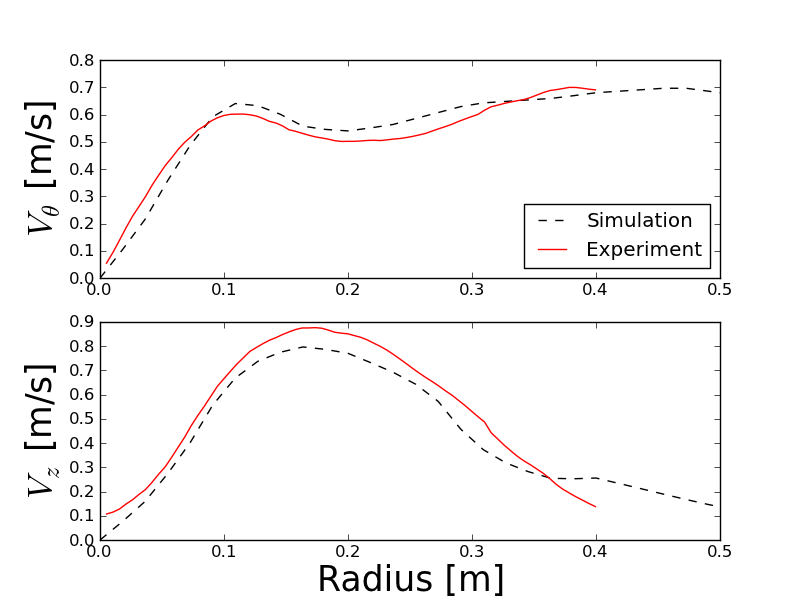
\includegraphics[width = 12 cm]{figs/hybrid_profile}
   \caption{Azimuthal and vertical velocity profiles as a function of
   radius. The simulation and experimental data broadly agree, with
   the simulation also exhibiting the characteristic ``twin-peak''
   structure of the hybrid vanes in the azimuthal velocity. }
   \label{fig:lab}
  \end{center}
\end{figure}


\todo{finish me}